\textbf{Determina el volumen del cilindro de la figura \ref{fig:vol_cil_07}.}\\
\textit{Ingresa una respuesta exacta en términos de $\pi$, o usa 3.14.}\\

\begin{minipage}[t]{0.3\linewidth}
    \begin{figure}[H]
        \centering
        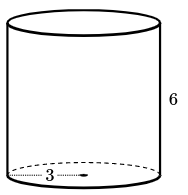
\includegraphics[width=0.75\textwidth]{../images/vol_cil_07.png}
        \caption{}
        \label{fig:vol_cil_07}
    \end{figure}
\end{minipage}%
\begin{minipage}[t]{0.7\linewidth}
    \begin{solutionbox}{5cm}        El volumen de un cilindro de radio $r$ y altura $h$ es:
        \begin{equation*}
            V = \pi r^2 h
        \end{equation*}
        De la figura \ref{fig:vol_cil_07} se sabe que $r=2$ y $h=5$, entonces
        \begin{equation*}
            \begin{split}
                V & = \pi r^2 h\\
                & = \pi (3)^2 (6)\\
                & = \pi (9) (6)\\
                & = 54\pi
            \end{split}
        \end{equation*}
    \end{solutionbox}
\end{minipage}%